%%%%%%%%%%%%%%%%%%%%%%%%%%%%%%%%%%%%%%%%%%%%%%%%%%%%%%%%%%%%%%%%%%%%%
% BY MAHAMDI AMINE
%%%%%%%%%%%%%%%%%%%%%%%%%%%%%%%%%%%%%%%%%%%%%%%%%%%%%%%%%%%%%%%%%%%%%%
\documentclass[12pt]{report}
\usepackage[T1]{fontenc}
\usepackage{lmodern}
\usepackage[a4paper]{geometry}
\usepackage[myheadings]{fullpage}
\usepackage{fancyhdr}
\usepackage{lastpage}
\usepackage{graphicx, wrapfig, subcaption, setspace, booktabs}
\usepackage[T1]{fontenc}
\usepackage[font=small, labelfont=bf]{caption}
\usepackage[protrusion=true, expansion=true]{microtype}
\usepackage[french,english]{babel}
\usepackage{sectsty}
\usepackage{hyperref}
\hypersetup{
    colorlinks,
    citecolor=black,
    filecolor=black,
    linkcolor=black,
    urlcolor=black
}
\usepackage{url, lipsum}
\usepackage[utf8]{inputenc}
\usepackage{indentfirst}
\newcommand{\HRule}[1]{\rule{\linewidth}{#1}}
\onehalfspacing
\setcounter{tocdepth}{5}
\setcounter{secnumdepth}{5}

%-------------------------------------------------------------------------------
% HEADER & FOOTER
%-------------------------------------------------------------------------------
\pagestyle{fancy}
\fancyhf{}
\setlength\headheight{15pt}
\fancyhead[L]{fm\char`_mahamdi@esi.dz    }
\fancyhead[R]{fn\char`_adrao@esi.dz}
\fancyfoot[R]{Page \thepage\ sur \pageref{LastPage}}
\usepackage{placeins}
%-------------------------------------------------------------------------------
% TITLE PAGE
%-------------------------------------------------------------------------------

\begin{document}
	\renewcommand{\contentsname}{Table des Matières}
\renewcommand{\listfigurename}{Table des Figures}

	\author{MAHAMDI Mohammed & ADRAO Nassim}        
	\date{} 
	\title{  \textsc{ Le problème du Sac à dos}
		\\ [2.0cm]
		\HRule{0.5pt} \\
		\LARGE \textbf{\uppercase{Rapport de TP1 }}
		\HRule{2pt} \\ [0.5cm]
		\normalsize \today \vspace*{5\baselineskip}}
	\maketitle
	\tableofcontents
\newpage
\listoffigures 
	\newpage
	%------------------------------------------------------------------------------
	% Section title formatting
	\sectionfont{\scshape}
	
	%------------------------------------------------------------------------------
	% introduction
	%------------------------------------------------------------------------------
	%\newpage
	\chapter{Introduction}
	%\section{Introduction}
	% \addcontentsline{toc}{section}{Introduction}
	 %\par{}
	 En algorithmique, le problème du sac à dos, noté également KP (en anglais, Knapsack problem) est un problème d'optimisation combinatoire. Il modélise une situation analogue au remplissage d'un sac à dos, ne pouvant supporter plus d'un certain poids, avec tout ou partie d'un ensemble donné d'objets ayant chacun un poids et une valeur. Les objets mis dans le sac à dos doivent maximiser la valeur totale, sans dépasser le poids maximum.
	\section{Approche de solution}
%\addcontentsline{toc}{section}{Introduction}
\par{}
	Pour résoudre ce problème, on peut utiliser la solution classique ou glouton consistant à essayer tous les cas possible. Cela est innéficace pour des valeurs de n supérieur à 8 par exemple.
\par{}
	C'est pour cela que la programmation dynamique est la solution la plus adéquate, et c'est le but de ce TP1.
	
	\section{Principe de la programmtion dynamique}
	La solution récursive est la plus évidente mais la plus coûteuse, la programmation dynamique est par conséquent une amélioration qui consiste à sauvegarder les valeurs des transitions déja calculer pour ne pas répéter les calculs inutile.
	\par{}
	Il existe deux approches:
	\begin{itemize}
		\item \textbf {Approche ascendante}:
		Pour calculer le n ième élément, on commence par calculer le premier élément, puis le deuxième, ... jusqu'à arriver au dernier élément.
		\item \textbf {Approche descendante}:
		Pour calculer le n ième élément, on calcule l'élément n-1 , puis l'élément n-2 , ... jusqu'à arriver au premier élément.
		
	\end{itemize}	
	
	\chapter{Implémentation de la solution}
	\section{Approche choisie}
	On a utilisé l'approche ascendante (voir introduction)
	\section{Les équations de récurrence}
	\[
    P_{ij}=\left\{
                \begin{array}{ll}
                  0 $ si $ i=0$ ou $j=0\\
                  P_{i-1j} $ si $ j<w_{i} , i>0\\
                  \max\lbrace P_{i-1,j}, P_{i-1,j-w_{i}}+v_{i} \rbrace
                \end{array}
              \right.
  \]
	\section{Processus}\begin{enumerate}
		\item On lit la capacité du sac à dos, nommée \emph{maxWeight}.
		\item On lit n objets et pour chaque objet on introduit le poids et le gain correspondant sous forme de tableau comme le montre la figure suivante:
		\item On construit une matrice nommée \emph{matrix} de n+1 lignes (la 1 ère ligne d'indice 0 contient des 0 partout, utile juste pour l'utiliation des équations de réferrence) et maxWeight+1 colone (la 1 ère colone d'indice 0 contient des 0 partout, utile juste pour l'utiliation des équations de réferrence)
		\item On remplit cette matrice en utilisant les équations de référence (voir section 2.2).
		\item après la rempli de cette matrice , on trouve le gain maximum dans \emph{matrix[n][maxWeight]}.
		\item Pour la recherche des objets choisis, on procède à la comparaison des valeurs de la dernière colonne comme suit
		\begin{enumerate}
		\item On initialise un pointeur entier k à n, et un pointeur col à  maxWeight.
		\item on compare le gain matrix[k][col] avec matrix[k+1][col].
		\item si matrix[k][col] != matrix[k+1][col] alors élément k choisi
		\item Soustraire le poids $w_{i}$de l'élément choisi de col, on décrémente le k et si k != 1 aller à 2.
		\end{enumerate}
	\end{enumerate}
	\par{}
	Les figures suivantes montrent les résultats de l'implémentation :
	\begin{figure}[hp]
\centering
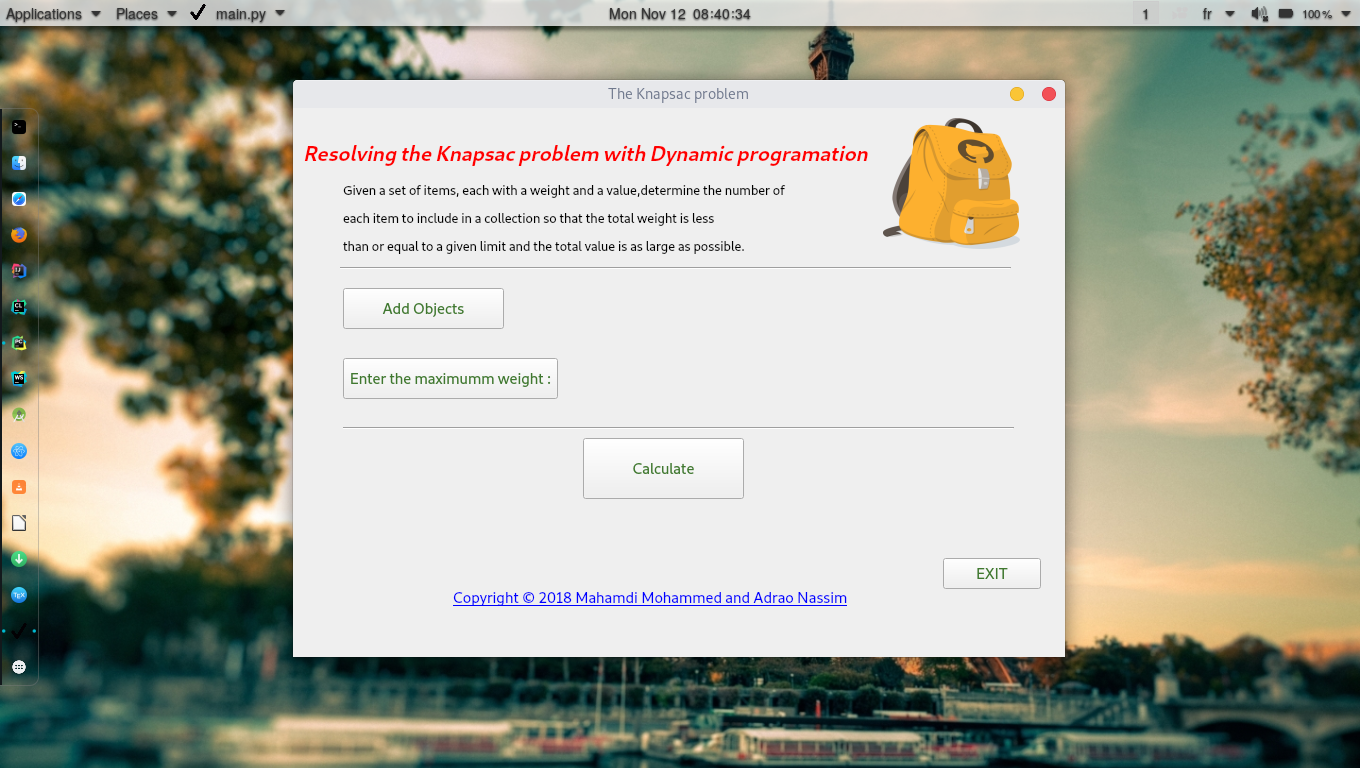
\includegraphics[scale=1, width=18cm]{../screenshots/1.png}
	\caption{Page d'acceuil}
	\end{figure}
\begin{figure}[h!]
	\centering
	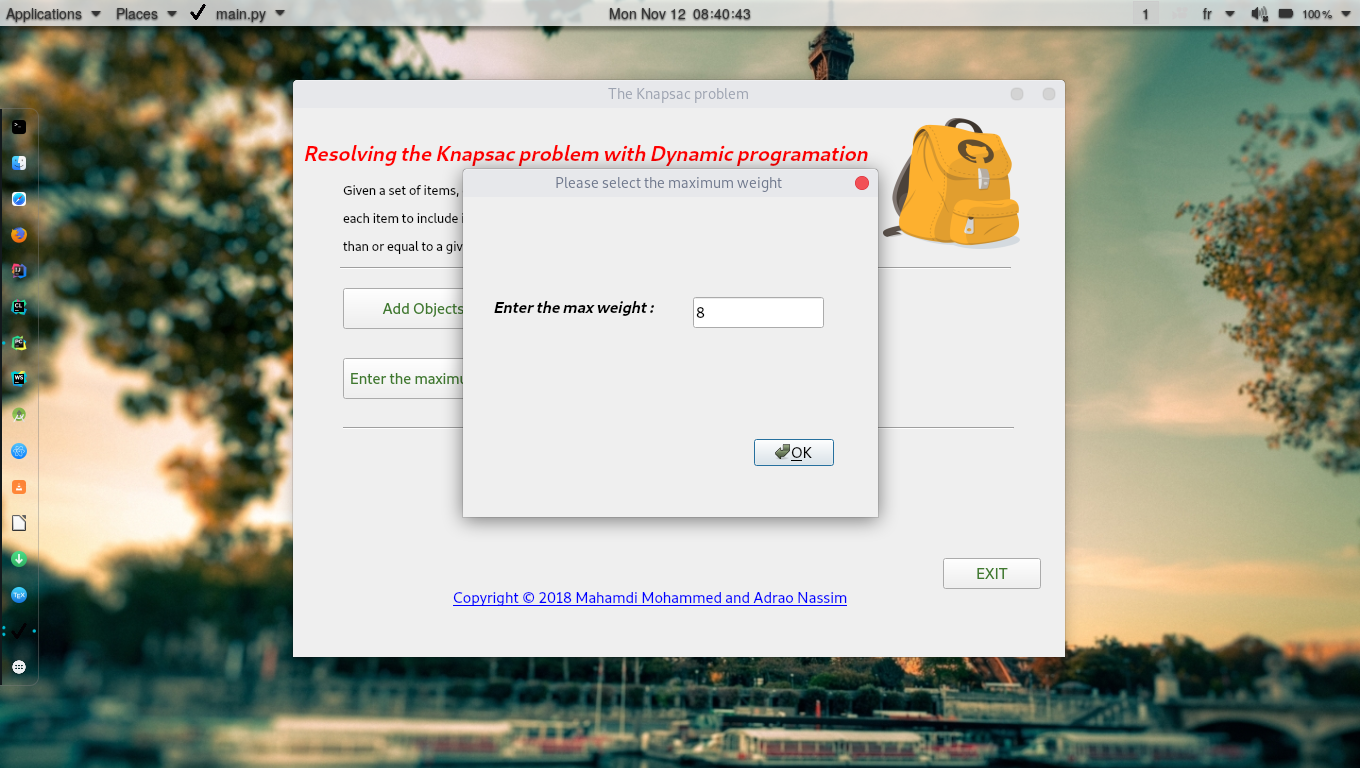
\includegraphics[scale=1, width=18cm]{../screenshots/2.png}
	\caption{Saisie de la taile de sac à dos}	
	\end{figure}
	\begin{figure}[h!]
	\centering
	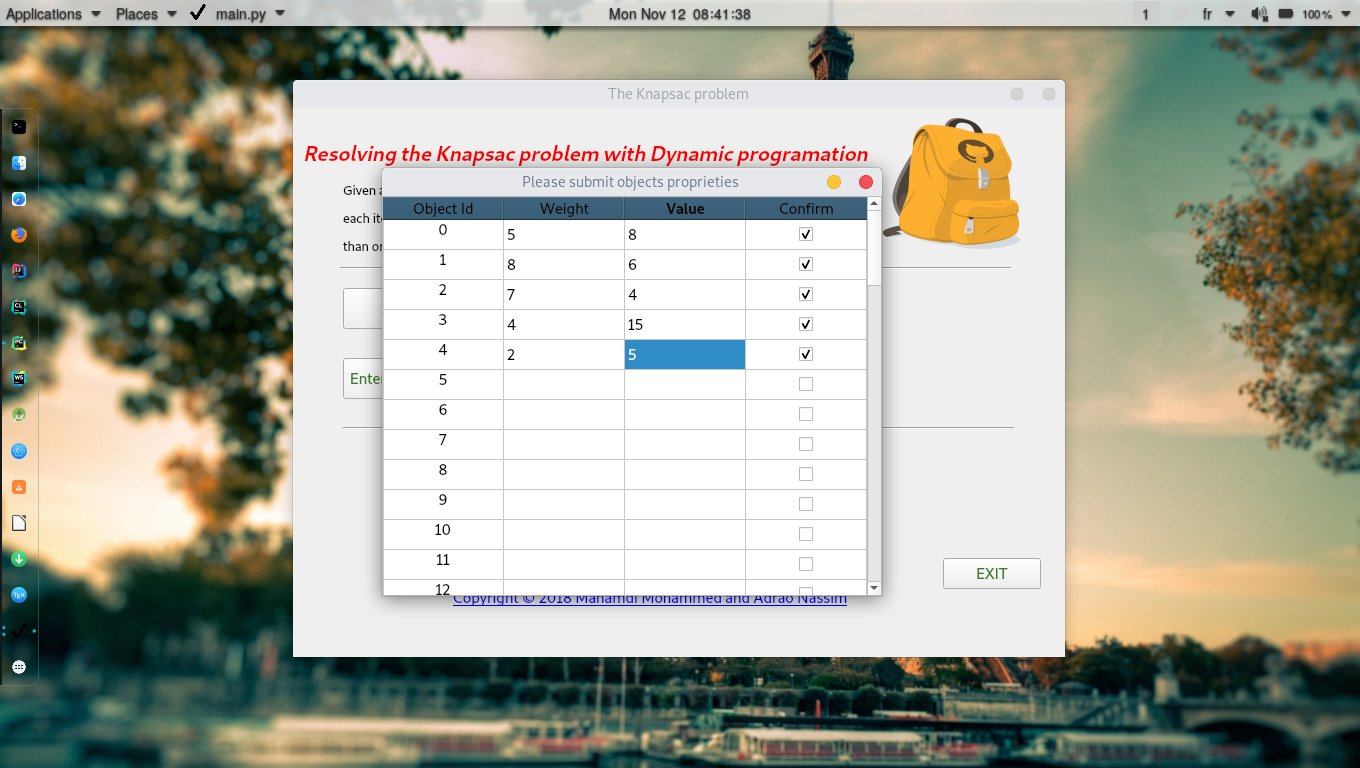
\includegraphics[scale=1, width=18cm]{../screenshots/3.png}
	\caption{Saisie des donnée concernant les objets}
	\end{figure}
	\begin{figure}[h!]
	\centering
	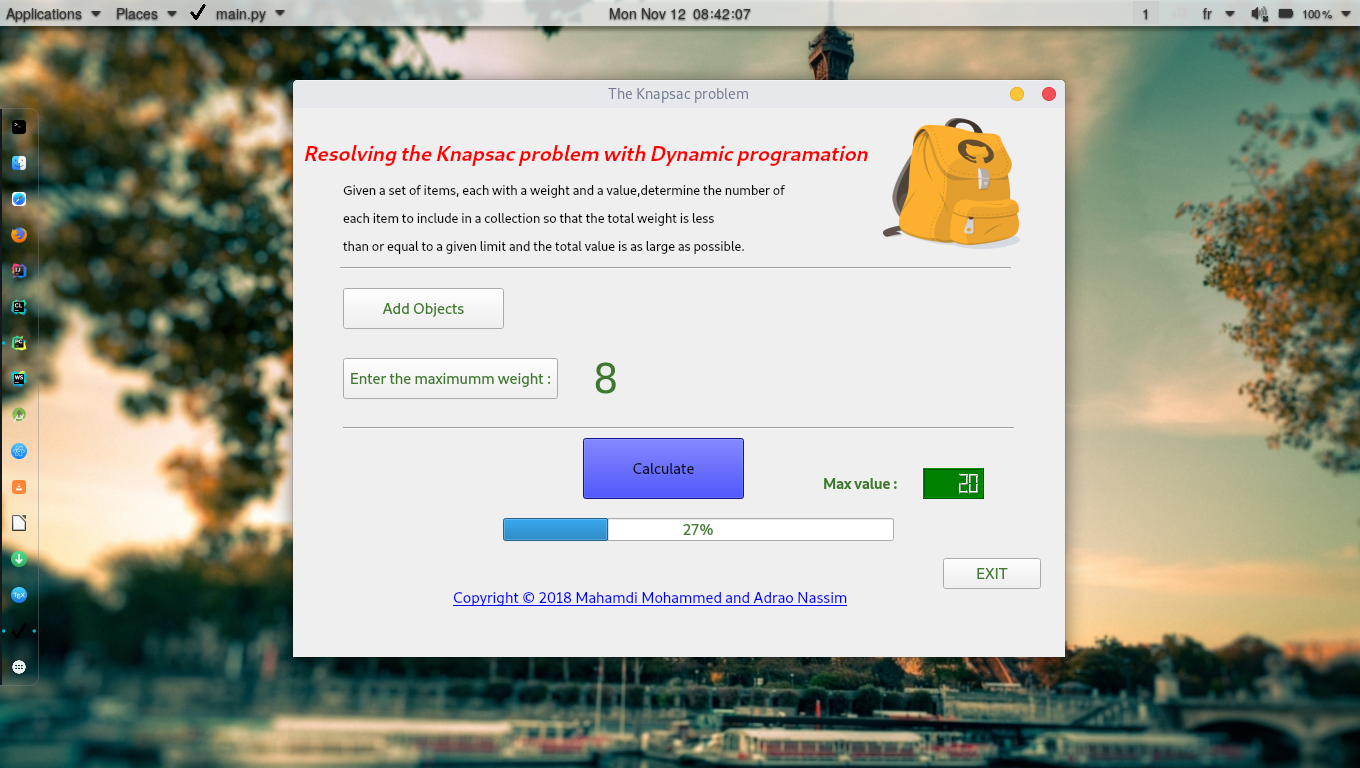
\includegraphics[scale=1, width=18cm]{../screenshots/4.png}
	\caption{Calcul de gain maximal}
	\end{figure}
	\begin{figure}[h!]
	\centering
	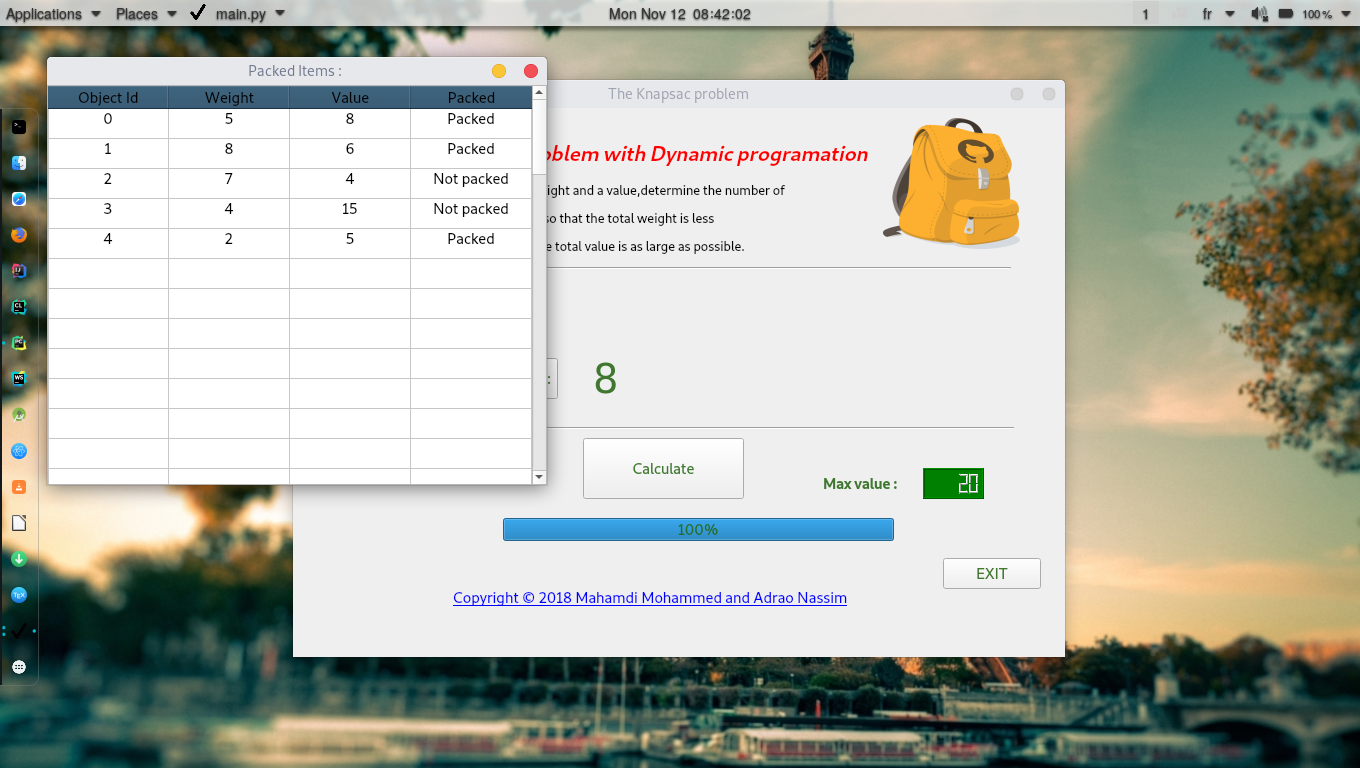
\includegraphics[scale=1, width=18cm]{../screenshots/5.png}
	\caption{Affichage d'une combinaison des éléments choisi satisfaisant les contraintes}
	\end{figure}
	\newpage	
	\FloatBarrier
	\section{Calcul de la complexité}
	\par{} 
	
	La complexité de l'algorithme : O($m^{2}$)
	%\subsection{preuve}
	
	\paragraph*{preuve}:
	On doit remplir la matrice de n lignes et p colonnes, don la complexité est O($m^{2}$) tel que m=max(n,p); 	Puis on parcourt la dernière colonne (complexité= O(n)) n est le nombre de lignes
	\par{}
	Donc la complexité finale sera : max(O($m^{2}$), O(n)) = $O(m^{2})$
	\chapter{Conclusion}
	\par{} 
	La programmation dynamique sert à résoudre de très grand nombre de problèmes, on remarque cela dans ce TP.
\par{}	
	La complexité de la programmation dynamique est polynomial tout en gardant la simplicité de la récursivité avec une complexité base
	\par{}
	La programmation dynamique est un cas de l'intelligence artificielle 
	\par{}
	Le problème de sac à dos est l'un des problèmes classiques en informatique, qui reste jusqu'ici valable pour les problèmes qui sont résolu en conséquent.

\end{document}
